\documentclass[a4paper]{article}

\usepackage[lmargin=25mm,rmargin=25mm,tmargin=25mm,bmargin=25mm]{geometry}
\usepackage{amsmath, amssymb}
\usepackage{babel}
\usepackage{hyperref}
\usepackage{xcolor}
\usepackage{graphicx}

\title{RoboCup 2024 \\ Standard Platform League (SPL) \\ Technical Challenge \\ --- \textsc{Shared Autonomy} --- \\\vspace{2cm} 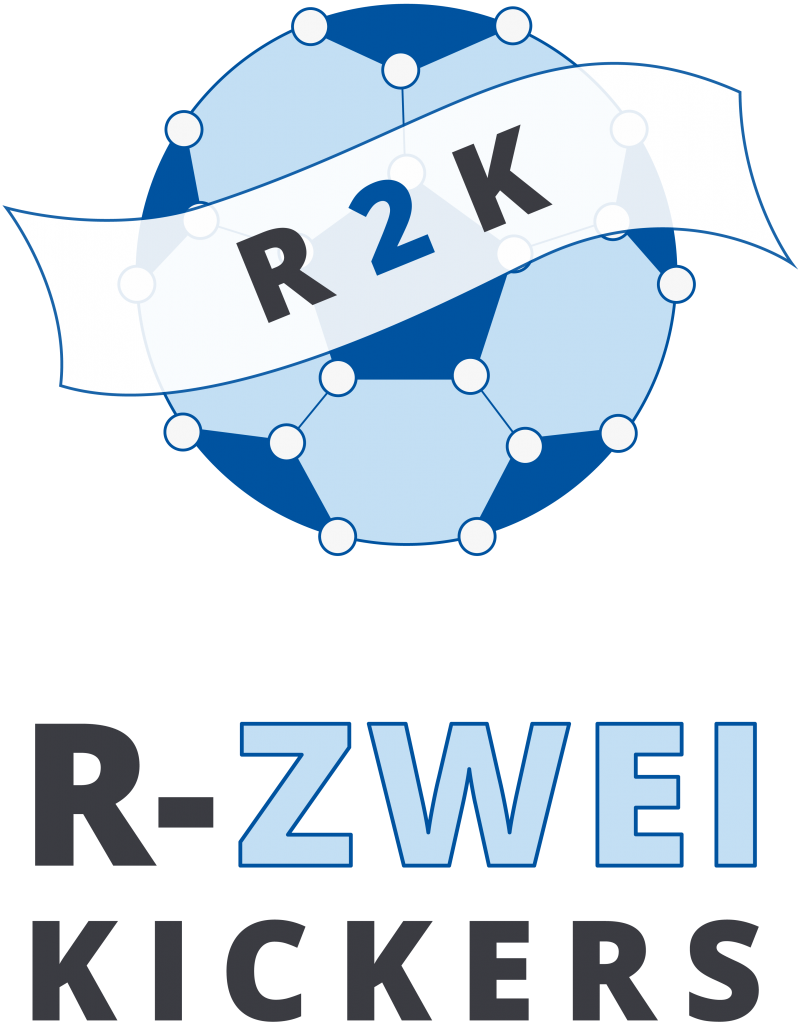
\includegraphics[width=0.5\textwidth]{img/R2K_Logo}}
\date{last updated: \today}
\author{Adrian Müller \\ Desmond Krämer \\ Samuel Njike Megaptche \\ Thomas Jäger \\ Wilhelm Simus}

\begin{document}
	\setlength{\parindent}{0pt}
	\pagestyle{empty}
	\maketitle
	%\newpage
	%\tableofcontents
	\newpage
	\pagestyle{headings}
	
	\section{The Challenge 2024: Shared Autonomy}
	
	In the 2024 technical challenge, the teams have to develop a mixed team that consists of one human-operated Nao robot and one fully autonomous Nao.
	This challenge will consist of matches of two vs two robots on the standard SPL field. 
	
	\subsection{The Goal}
	
	This challenge takes a step towards the goal of enabling robots to play on the same field as agents with human level intelligence.
	To level the playing field in terms of physical embodiment, all players will be Nao robots.
	However, each team will have one of their robots be remotely operated by a human to provide human-level intelligence for robot control.
	The other robot will be fully autonomous in accordance with the main SPL competition rules.\\
	
	For further references and exact rules, see \href{https://spl.robocup.org/wp-content/uploads/SPL-Challenges-2024.pdf}{\textcolor{blue}{the official challenge rules}} provided by the technical committee.
	
	\section{Our approach}
	
	- We have web app / interface / browser\\
	- Backend: communicates with robot via TCP\\
	- ...\\
	- send byte commands to robot\\
	- on robot side: module for receiving and interpreting human OP commands\\
	
	\begin{figure}[h]
		\centering
		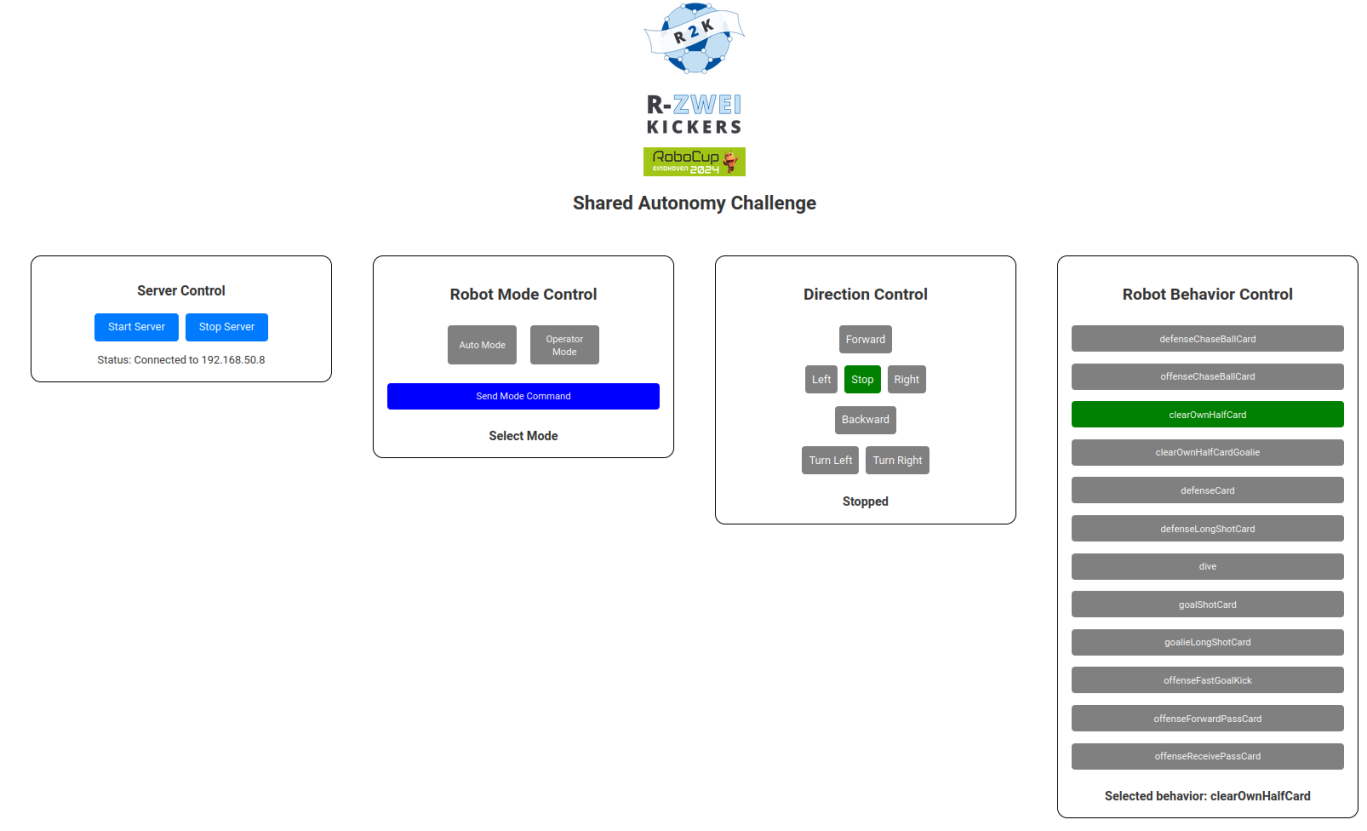
\includegraphics[width=\textwidth]{img/SAC}
		\caption{The Interface for the shared autonomy challenge consists of four distinct Control modules}
	\end{figure}
	
	\subsection{Tactical Overview}
	
	- Robot Mode Control (allows toggling between autonomous walk and full human control)\\
	- Direction Control: Interface for full human walk control\\
	- Behavior Control: manual card selection from behavior stack (BHuman skills and cards framework)\\
	
	\subsection{Technical Overview}
	
	- Frontend: Minimalist Web-App based on Svelte\\
	- Backend: Python Flask Server\\
	- works like REST-interface using endpoints for different control interfaces\\
	- Server converts commands from frontend to byte-msgs and sends them to the bot\\
	- On robot side there's a module which interprets the byte msgs and writes the commands in the representation, s.t. other modules can gather/use/access this information and cards or skills can be parameterized
	
	\section{Future Enhancements}
	
	- Fine tuning of inter-robot comms: trigger sending msgs from one bot to another\\
	- better tactics / more flashed out tactical view
	
	
\end{document}